%!TEX root=writeup.tex
\section{Evaluation}
For evaluation, we tested the effectiveness of our prototype implementation 
on six different SQL rewriting rules.
We mainly focused on three aspects in the evaluation:
\begin{itemize}
\item Whether our prototype can prove the correctness of rewriting rules.
\item Whether our prototype can find erros in wrong rewrting rules.
\item How does our prototype scale with the size of the symbolic schema.
\end{itemize}

\subsection{Proving Rewriting Rules on Bounded schema}
\subsection{Detecting Incorrect Rewriting Rules}
\subsection{Scalability of our Prototype}
To illustrate the scalability of our prototype implementation, we evaluated
6 rewriting rules with different symbolic schema sizes on a desktop PC
~\footnote{The PC has 3.60GHz Intel Core i7 CPU, and 8 GB of memeory}.
Figure XXX shows the time it takes to verify the equivalence of SQL queries
with different symbolic schema sizes.

\begin{figure}[!htb]
  \centering
  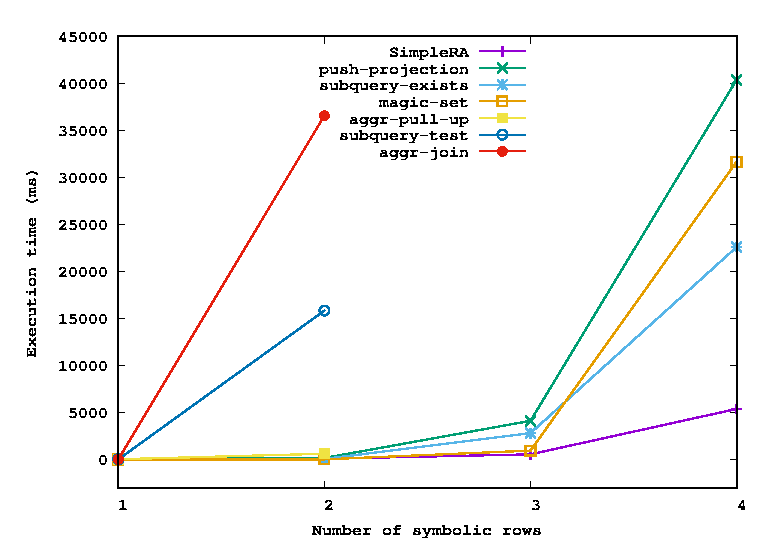
\includegraphics[width=0.7\linewidth]{scale.eps}
  \caption{\# of Symbolic Rows v. Verification Execution Time}
  \label{fig:scale}
\end{figure}

From the figure, we can see that the scalability of the verifier heavily depends 
on the complexity of the rewriting rules.
For those rewriting rules without table join and subquery, it can scales pretty well.
For rewriting rules with either table join or subquery, the prototype implementation can 
not scale well with the growing of the size of the symbolic schema.
Based on our evaluation, queries with both table join and subquery can not scale to schema with
more than 2 rows.
